\documentclass{article}

\def\ParSkip{} 
% Packages
\usepackage{amssymb,amsmath,amsthm,bbm}
\usepackage{verbatim,float,url,dsfont}
\usepackage{graphicx,subfigure,psfrag}
\usepackage{algorithm,algorithmic}
\usepackage{mathtools,enumitem}
\usepackage{multirow}
\usepackage{ragged2e}
\usepackage{xr-hyper}
\usepackage{array}

\usepackage[colorlinks=true,citecolor=blue,urlcolor=blue,linkcolor=blue]{hyperref}
\usepackage[margin=1in]{geometry}
\usepackage[round]{natbib}

\usepackage[utf8]{inputenc} % allow utf-8 input
\usepackage[T1]{fontenc}    % use 8-bit T1 fonts
\usepackage{booktabs}       % professional-quality tables
\usepackage{nicefrac}         % compact symbols for 1/2, etc.
\usepackage{microtype}      % microtypography

\ifdefined\TimesFont 
\usepackage{times} % use times font
\fi

\ifdefined\ParSkip 
\usepackage{parskip} % use par skip
\fi

% Theorems and such
\newtheorem{theorem}{Theorem}
\newtheorem{lemma}{Lemma}
\newtheorem{corollary}{Corollary}
\newtheorem{proposition}{Proposition}
\theoremstyle{definition}
\newtheorem{remark}{Remark}
\newtheorem{definition}{Definition}

% Assumption
\newtheorem*{assumption*}{\assumptionnumber}
\providecommand{\assumptionnumber}{}
\makeatletter
\newenvironment{assumption}[2]{
  \renewcommand{\assumptionnumber}{Assumption #1#2}
  \begin{assumption*}
  \protected@edef\@currentlabel{#1#2}}
{\end{assumption*}}
\makeatother

% Widebar
\makeatletter
\newcommand*\rel@kern[1]{\kern#1\dimexpr\macc@kerna}
\newcommand*\widebar[1]{%
  \begingroup
  \def\mathaccent##1##2{%
    \rel@kern{0.8}%
    \overline{\rel@kern{-0.8}\macc@nucleus\rel@kern{0.2}}%
    \rel@kern{-0.2}%
  }%
  \macc@depth\@ne
  \let\math@bgroup\@empty \let\math@egroup\macc@set@skewchar
  \mathsurround\z@ \frozen@everymath{\mathgroup\macc@group\relax}%
  \macc@set@skewchar\relax
  \let\mathaccentV\macc@nested@a
  \macc@nested@a\relax111{#1}%
  \endgroup
}
\makeatother

% Min and max
\newcommand{\argmin}{\mathop{\mathrm{argmin}}}
\newcommand{\argmax}{\mathop{\mathrm{argmax}}}
\newcommand{\minimize}{\mathop{\mathrm{minimize}}}
\newcommand{\maximize}{\mathop{\mathrm{maximize}}}
\newcommand{\st}{\mathop{\mathrm{subject\,\,to}}}

% Shortcuts
\def\R{\mathbb{R}}
\def\C{\mathbb{C}}
\def\Z{\mathbb{Z}}
\def\N{\mathbb{N}}
\def\E{\mathbb{E}}
\def\P{\mathbb{P}}
\def\T{\mathsf{T}}
\def\Cov{\mathrm{Cov}}
\def\Var{\mathrm{Var}}
\def\indep{\perp\!\!\!\perp}
\def\th{^{\text{th}}}
\def\tr{\mathrm{tr}}
\def\df{\mathrm{df}}
\def\dim{\mathrm{dim}}
\def\col{\mathrm{col}}
\def\row{\mathrm{row}}
\def\nul{\mathrm{null}}
\def\rank{\mathrm{rank}}
\def\nuli{\mathrm{nullity}}
\def\spa{\mathrm{span}}
\def\sign{\mathrm{sign}}
\def\supp{\mathrm{supp}}
\def\diag{\mathrm{diag}}
\def\aff{\mathrm{aff}}
\def\conv{\mathrm{conv}}
\def\dom{\mathrm{dom}}
\def\hy{\hat{y}}
\def\hf{\hat{f}}
\def\hmu{\hat{\mu}}
\def\halpha{\hat{\alpha}}
\def\hbeta{\hat{\beta}}
\def\htheta{\hat{\theta}}
\def\cA{\mathcal{A}}
\def\cB{\mathcal{B}}
\def\cD{\mathcal{D}}
\def\cE{\mathcal{E}}
\def\cF{\mathcal{F}}
\def\cG{\mathcal{G}}
\def\cK{\mathcal{K}}
\def\cH{\mathcal{H}}
\def\cI{\mathcal{I}}
\def\cL{\mathcal{L}}
\def\cM{\mathcal{M}}
\def\cN{\mathcal{N}}
\def\cP{\mathcal{P}}
\def\cS{\mathcal{S}}
\def\cT{\mathcal{T}}
\def\cW{\mathcal{W}}
\def\cX{\mathcal{X}}
\def\cY{\mathcal{Y}}
\def\cZ{\mathcal{Z}}


\title{High-Dimensional Regression: Lasso \\ \smallskip
\large Advanced Topics in Statistical Learning, Spring 2023 \\ \smallskip
Ryan Tibshirani}
\date{}

\begin{document}
\maketitle
\RaggedRight
\vspace{-50pt}

\section{Introduction}

In this lecture, we'll move on from low-dimensional nonparametric to
high-dimensional parametric regression. Though this might seems like very  
different problems, as we'll see, they do share some similarities.

Below, we provide a quick recap of what we know about least squares and
motivations for regularization (as also covered in the review lecture), laying
the groundwork for the main estimators we'll study in this and the next lecture
on high-dimensional regression: lasso and ridge.  

\subsection{Recap: least squares regression}

Suppose we are given $n$ observations of the form $(x_i, y_i)$, $i=1,\dots,n$
where each $x_i \in \R^d$ denotes a feature vector and $y_i \in \R$ an
associated response value. Let $X \in \R^{n \times d}$ denote the predictor
matrix (whose $i\th$ row is $x_i$) and $Y \in \R^n$ denote the response 
vector. Recall that the least squares regression coefficients of $Y$ on $X$ are
given by solving  
\begin{equation}
\label{eq:ls}
\minimize_\beta \; \|Y - X\beta\|_2^2.
\end{equation}
When $d \leq n$ and $\rank(X) = d$, this produces the unique solution 
\[
\hbeta = (X^\T X)^{-1} X^\T Y.  
\]
The fitted values (i.e., in-sample predictions) are 
\[
X\hbeta = X (X^\T X)^{-1} X^\T Y = P_X Y,
\]
where $P_X = X (X^\T X)^{-1} X^\T $ denotes the projection onto the column space
of $X$. 

\paragraph{Risk properties.}

Now let's recall the risk properties of least squares. Assume $(x_i,y_i)$,
$i=1,\dots,n$ are i.i.d.\ such that $X^\T X$ is almost surely invertible, and 
\[
y_i = x_i^\T \beta_0 + \epsilon_i, \quad i=1,\dots,n,
\]
where $\epsilon_i$ has mean zero and variance $\sigma^2$, and $\epsilon_i \indep
x_i$. Note that we can equivalently write this as 
\begin{equation}
\label{eq:model}
Y = X\beta_0 + \epsilon.
\end{equation}
The in-sample prediction risk of least squares is
\begin{equation}
\label{eq:ls_risk_in}
\frac{1}{n} \E \big[ \| X\hbeta - X\beta_0 \|_2^2 \,|\, X \big] = \sigma^2
\frac{d}{n}.  
\end{equation}
Meanwhile, the out-of-sample prediction risk is
\begin{equation}
\label{eq:ls_risk_out}
\E \big[ (x_0^\T\hbeta - x_0^\T\beta_0 )^2 \big] = \sigma^2 \tr\Big(\E [x_0
x_0^\T] \, \E [(X^\T X)^{-1}] \Big) \approx \sigma^2 \frac{d}{n-d},
\end{equation}
where the expectation is taken over the training data $(x_i,y_i)$, $i=1,\dots,n$
and an independent draw $x_0$ from the predictor distribution.  The middle 
expression above is an equality in general. The rightmost expression is an
approximation that holds as $n,d$ grow large in a random matrix theory model,
which we'll learn the details of when we study ridge regression. (Further, the
rightmost expression is exact for Gaussian features.)

\subsection{Recap: trouble in high dimensions}

As we just saw in \eqref{eq:ls_risk_in}, \eqref{eq:ls_risk_out}, the risk of
least squares regression degrades as $d$ grows close to $n$---and looking at the
rightmost expression in \eqref{eq:ls_risk_out}, the out-of-sample risk actually
diverges at $d=n$.

Meanwhile, the least squares estimator itself is not even well-defined when $d >
n$, in that the optimization problem \eqref{eq:ls} does not have a unique
solution. In this case, any vector of the form 
\begin{equation}
\label{eq:ls_eta}
\hbeta = (X^\T X)^+ X^\T Y + \eta, \quad \text{where $\eta \in \nul(X)$},
\end{equation}
solves \eqref{eq:ls}, where we write $A^+$ to denote the generalized inverse of
a matrix $A$, and $\nul(A)$ to denote its null space.

If all we care about is out-of-sample prediction, then this is not the end of
the story for least squares---it turns out that taking $\eta=0$ in
\eqref{eq:ls_eta}, which yields the \emph{minimum $\ell_2$ norm least squares
  solution}, can still have interesting predictive properties when $d>n$. We'll
study this later, in the overparametrization lecture.   

But if we additionally care about the estimated coefficients themselves, then it
really is the end of the road for least squares. This is because, for any
\smash{$\hbeta$} of the form \eqref{eq:ls_eta} with \smash{$\hbeta_j > 0$} for
some component $j$, we can always find\footnote{Technically, this is only true
  if $\nul(X) \not\perp e_j$, where $e_j$ is the $j\th$ standard basis
  vector. Note that the latter condition must hold for at least one $j$, as
  $\nul(X) = \{0\}$. And for random features, under very weak conditions, it
  will be true almost surely for any $j$.} 
another \smash{$\tilde\beta$} of the form \eqref{eq:ls_eta} with
\smash{$\tilde\beta_j < 0$}. So we cannot even consistently interpret the sign
of any estimated coefficient (let alone its magnitude). 

\subsection{Recap: regularization to the rescue}

Regularization will finesse the problems described above. At a high level, it
gives us a way to produce nontrivial coefficient estimates, and it may well give 
us better predictions as well. (It typically does, and most people would have
traditionally said that it pretty much \emph{always} does. However, recent
developments in overparametrization have shown us that there is more nuance to 
the prediction story, and whether or not explicit regularization helps depends
very strongly on the operating characteristics of the prediction problem.) 

In the least squares setting, traditional approaches for regularization take two
forms:  
\begin{alignat*}{3}
&\text{Constrained form}: \quad 
&&\minimize_\beta \; \|Y - X\beta\|_2^2 \;\; \st \;\; \beta \in C \\
&\text{Penalized form}: \quad 
&&\minimize_\beta \; \|Y - X\beta\|_2^2 + h(\beta).
\end{alignat*}
Here $C$ is some (typically convex) set, and $h$ is some (typically convex)
penalty function. Typically $C = \{\beta : \|\beta\| \leq t\}$ is the sublevel
set of a norm $\|\cdot\|$, and $h(\beta) = \lambda \|\beta\|$ is a nonnegative
multiple of a norm. In this case, the constrained and penalized forms can be 
seen to equivalent, via convex duality: that is, for any $t \geq 0$ and solution 
\smash{$\hbeta$} in the constrained problem, there is a value of $\lambda \geq
0$ such that \smash{$\hbeta$} also solves the penalized problem, and vice
versa. 

We'll mostly focus on the penalized form in this lecture, since it is generally
more commonly studied, but we'll also cover the constrained form when we work
out prediction and estimation theory. 

\paragraph{Canonical regularizers: $\ell_0$, $\ell_1$, and $\ell_2$.}

In regression, arguably the three canonical choices for regularizers are the
$\ell_0$, $\ell_1$, and $\ell_2$ norms: 
\[
\|\beta\|_0 = \sum_{j=1}^d 1\{\beta_j \not= 0\}, \;\;\;
\|\beta\|_1 = \sum_{j=1}^d |\beta_j|, \;\;\;
\|\beta\|_2 = \bigg(\sum_{j=1}^d \beta_j^2 \bigg)^{1/2}.
\]
This gives rise to what we call best subset selection, the lasso, and ridge
regression. In the current lecture we'll focus on the lasso, and in the next
we'll focus on ridge regression.

Calling $\|\cdot\|_0$ the ``$\ell_0$ norm'' is a misnomer, since it is not
actually a norm: it does not satisfy positive homogeneity, i.e., $\|a\beta\|_0 = 
a\|\beta\|_0$ for all $a>0$. (As such, it would be more accurate to call it the
``$\ell_0$ pseudonorm'', but in keeping with common convention, we'll simply use
``norm''.)    

Critically, $\|\cdot\|_0$ is \emph{not convex}, while $\|\cdot\|_1$ and
$\|\cdot\|_2$ are (indeed, any norm is a convex function). This makes best
subset selection a nonconvex problem, and one that is generally very hard to
solve in practice except for very small $d$. On the other hand, the lasso and
ridge regression problems are convex, and many efficient algorithms exist for
them.    

\section{Lasso basics}

This section covers some basic properties of the \emph{least absolute selection
  and shrinkage operator} or lasso, defined by   
\begin{equation}
\label{eq:lasso}
\minimize_\beta \; \frac{1}{2} \|Y - X\beta\|_2^2 + \lambda \|\beta\|_1, 
\end{equation}
for a tuning parameter $\lambda \geq 0$. (The factor of $\frac{1}{2}$ is just
for convenience.) We start off by recalling a central property that the lasso
has in common with best subset selection, which replaces $\|\cdot\|_1$ in
\eqref{eq:lasso} by  $\|\cdot\|_0$: they produce \emph{sparse} solutions, that
is, at their solutions \smash{$\hbeta$}, we will have   
\[
\hbeta_j = 0, \; \text{for many $j$}.
\]
Larger values of the tuning parameter $\lambda$ typically means sparser
solutions. Why care about sparsity? This is often desirable, for two reasons:
(i) it corresponds to performing variable selection in the fitted linear model
(providing a level of interpretability of what features may be important), and
(ii) it can often predict better (in situations where the underlying regression
function is well-approximated by a sparse linear model).

In constrast, the \emph{ridge regression} estimator, 
\begin{equation}
\label{eq:ridge}
\minimize_\beta \; \|Y - X\beta\|_2^2 + \lambda \|\beta\|_2^2, 
\end{equation}
has a generically dense solution (all nonzero components), for any $\lambda \geq
0$. The fact that sparsity arises in \eqref{eq:lasso} but not \eqref{eq:ridge}
is often explained using the ``classic'' picture, in Figure
\ref{fig:lasso_ridge} (which illustrates the problems in constrained form). We
can also see a clear difference in how they behave in the case of an orthogonal
predictor matrix $X$ (meaning $X^\T X = I$); in this case, the solutions in
\eqref{eq:lasso}, \eqref{eq:ridge} are 
\begin{align*}
\hbeta^{\text{lasso}} &= S_\lambda(X^\T Y), \\
\hbeta^{\text{ridge}} &= (X^\T Y) / (1+\lambda),
\end{align*}
respectively, where $S_\lambda$ is soft-thresholding operator at the level
$\lambda$ applied componentwise, which is defined as $S_\lambda(a) = \sign(a)
(|a| - \lambda)_+$.  

\begin{figure}[htb]
\centering
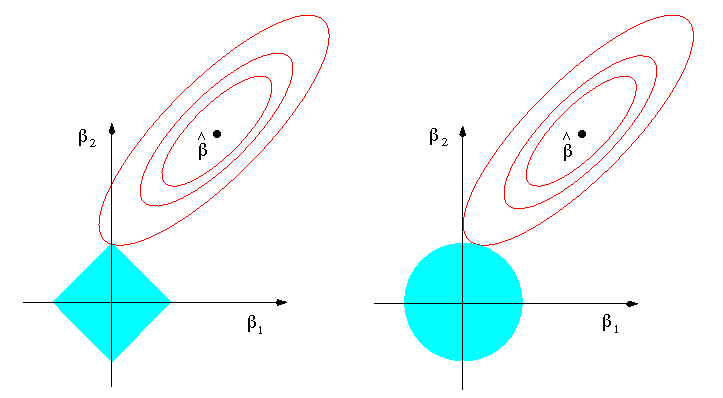
\includegraphics[width=0.95\textwidth]{lasso_ridge.pdf}
\caption{\it The ``classic'' illustration comparing lasso and ridge
  constraints. Credit: Chapter 3.4 of \citet{hastie2009elements}.}  
\label{fig:lasso_ridge}
\end{figure}

Another difference between the lasso \eqref{eq:lasso} and ridge \eqref{eq:ridge}
problems is that the latter is always strictly convex, whereas the former is not
strictly convex when $d>n$. This means that we are always guaranteed a unique
ridge solution, but not necessarily a unique lasso solution.   

Some basic convex analysis, as developed over the next few subsections, will
help us understand this better (and reveal that there is often not much to worry
about here). Our treament follows \citet{tibshirani2013lasso}.

\subsection{Sign consistency}

First, we make a basic observation: although the lasso solution is not always 
unique, the lasso fit \smash{$X\hbeta$} is always unique. This is true because 
the least squares loss $f(u) = \|Y - u\|_2^2$ is strictly convex in $u$. (Note
that the same is true of the least squares fit: it is always unique, even when
the solution is not.)

Next, consider the subgradient optimality condition (sometimes called the KKT 
condition) for the lasso problem \eqref{eq:lasso}, which is
\begin{equation}
\label{eq:lasso_kkt}
X^\T (Y - X\hbeta) = \lambda s,
\end{equation}
where \smash{$s \in \partial \|\hbeta\|_1$}, a subgradient of the $\ell_1$ norm
evaluated at \smash{$\hbeta$}. Precisely, 
\begin{equation}
\label{eq:lasso_sg}
s_j \in \begin{cases} 
\{+1\} & \hbeta_j > 0 \\
\{-1\} & \hbeta_j < 0 \\
[-1,1] & \hbeta_j = 0,
\end{cases}, \quad j=1,\dots,d.
\end{equation}
From \eqref{eq:lasso_kkt}, \eqref{eq:lasso_sg} we can read off a straightforward
but important fact: the optimal subgradient $s$ is always unique, for any
$\lambda>0$. This is because it is determined by the unique fitted value
$X\hbeta$.    

Why is this important? It tells us that even in the case when lasso solutions
are nonunique, \emph{any two solutions must always agree on the signs of common
  nonzero coefficients}. That is, we cannot have two solutions \smash{$\hbeta,
  \tilde\beta$} such that \smash{$\hbeta_j > 0$} but \smash{$\tilde\beta_j <
  0$}. In this sense, the lasso is already much better behaved than least
squares when $d>n$. The next subsection shows that a much stronger statement 
can be made about the lasso solution itself, when $d > n$.     

\subsection{Structure of solutions}

It is not hard to prove that the lasso solution is ``often'' unique even when $d
> n$. But first, we'll need to do a little bit of work to to learn about the
structure of lasso solutions (which should be interesting in its own right). 
Define the \emph{equicorrelation set}   
\[
E = \big\{ j \in \{1,\dots,d\} \,:\, |X_j^\T (Y - X\hbeta)| = \lambda \big\}.   
\]
This is the set of variables that achieves the maximum absolute inner product
(correlation, for standardized predictors) with the lasso residual vector
\smash{$Y - X\hbeta$}. Assuming $\lambda>0$, this is the same as 
\[
E = \big\{ j \in \{1,\dots,d\} \,:\, |s_j| = 1 \big\}. 
\]
The equicorrelation set $E$ is always unique (as \smash{$X\hbeta,s$} are
unique). Note that the set $E$ contains the support set---also called the
\emph{active set}, and denoted \smash{$A = \supp(\hbeta)$} of any lasso solution 
\smash{$\hbeta$}, because for $j \notin E$, we have $|s_j| < 1$, which implies
that \smash{$\hbeta_j = 0$} .   

Thus we can write \smash{$X\hbeta = X_E\hbeta_E$} for any lasso solution
\smash{$\hbeta$}, where \smash{$\hbeta_E$} denotes the components of
\smash{$\hbeta$} indexed by $E$, and $X_E$ denotes the columns of $X$ indexed by
$E$. The subgradient condition \eqref{eq:lasso_kkt} implies
\[
X_E^\T (Y - X_E \hbeta_E) = \lambda s_E,
\]
and solving this for \smash{$\hbeta_E$} gives  
\[
\hbeta_E = (X_E^\T X_E)^+ (X_E^\T Y - \lambda s_E) + \eta, 
\quad \text{where $\eta \in \nul(X_E)$}.
\]
From this we learn the following sufficient condition for uniqueness: \emph{if
  the equicorrelated predictors are linearly independent, $\rank(X_E) = |E|$,
  then the lasso solution is unique and given by}
\begin{equation}
\label{eq:lasso_unique}
\begin{aligned}
\hbeta_E &= (X_E^\T X_E)^{-1} (X_E^\T Y - \lambda s_E), \\
\hbeta_{-E} &= 0.
\end{aligned}
\end{equation}
(Here \smash{$\hbeta_{-E}$} denotes the components of \smash{$\hbeta$} indexed 
by $E^c = \{1,\dots,d\} \setminus E$.) Interestingly, we can see above that this
is a certain \emph{shrunken} least squares estimator on the active set $E$.    
 
\subsection{Uniqueness and saturation}

The previous subsection established that when $\rank(X_E) = |E|$, then the lasso
solution is unique. A short calculation will show us that when the columns of 
$X$ are in what is known as \emph{general position}, a very weak condition, then
it must be the case that $\rank(X_E) = |E|$, and so the lasso solution is
unique. We state and prove this next.    

\begin{proposition}
Assume that $X$ has columns $X_1,\dots,X_d \in \R^n$ that are in general
position. This means that for any $k < \min\{n,d\}$, indices $i_1,\dots,i_{k+1} 
\in \{1,\dots,d\}$, and signs $\sigma_1,\dots,\sigma_{k+1} \in \{-1,+1\}$, the 
affine span of $\sigma_1 X_{i_1}, \dots,\sigma_{k+1} X_{i_{k+1}}$ does not
contain any element of $\{\pm X_i : i \not= i_1,\dots,i_{k+1}\}$. Then for any
$Y \in \R^n$ and $\lambda>0$, the lasso problem \eqref{eq:lasso} has a unique
solution. 
\end{proposition}

\begin{proof}
We will prove that contrapositive. We assume the lasso solution is not unique,
thus $\rank(X_E) < |E|$, and will prove that this means the columns of $X$ are
not in general position. Since $\rank(X_E) < |E|$, there exists some $i \in E$
such that 
\[
X_i = \sum_{j \in E\setminus\{i\}} c_j X_j.
\]
Hence
\[
s_i X_i = \sum_{j \in E\setminus\{i\}} (s_i s_j c_j) \cdot (s_j X_j).
\]
By definition of the equicorrelation set, $X_j^\T r = s_j \lambda$ for any $j
\in E$, where \smash{$r = Y-X\hbeta$} is the lasso residual vector. Taking the
inner  product of both sides above with $r$, we get 
\[
\lambda = \sum_{j \in E\setminus\{i\}} (s_i s_j c_j) \lambda,
\]
and since $\lambda>0$,
\[
\sum_{j \in E\setminus\{i\}} (s_i s_j c_j) = 1.
\]
Therefore, denoting $a_j = s_i s_j c_j$ for $j \in E\setminus\{i\}$, we have
shown that
\[
s_i X_i = \sum_{j \in E\setminus\{i\}} c_j X_j,
a_j \cdot s_j X_j, \quad \text{and} \quad 
\sum_{j \in E\setminus\{i\}} a_j = 1,
\]
which means that $s_iX_i$ lies in the affine span of $s_jX_j$, $j \in
E\setminus\{i\}$. Note that we can assume without a loss of generality that  
$E\setminus\{i\}$ has at most $n$ elements, since otherwise we can simply repeat
the above arguments replacing $E$ by any one of its subsets with $n+1$
elements. This means that the columns of $X$ cannot be in general position,
which completes the proof. 
\end{proof}

The lasso problem is an intriguing example where we get a unique solution
without strict convexity. To emphasize just how weak the general position
assumption, we note that if the entries of $X$ have a density on $\R^{nd}$, then
it is not hard to show that $X$ has columns in general position almost surely.
To emphasize, this gives us the following corollary.      

\begin{corollary}
Assume that the entries of $X$ are drawn from some continuous distribution on
$\R^{nd}$. Then almost surely, for any $Y \in \R^n$ and $\lambda>0$, the lasso
problem \eqref{eq:lasso} has a unique solution.  
\end{corollary} 

Here is another intriguing property of the lasso. 

\begin{proposition}
For any $X \in \R^{n \times d}$, $Y \in \R^n$, and $\lambda>0$, there exists a 
solution in the lasso problem \eqref{eq:lasso} whose active set $A$ has at most 
$\min\{n,d\}$ elements. In particular, when the lasso is unique, this means it
must have at most $\min\{n,d\}$ nonzero components.  
\end{proposition}

This property is often called \emph{saturation} of the lasso solution. It can be
shown using Carath{\'e}odory's theorem. Note that it is not necessarily a good
thing---when we have, say, $d=10000$ variables and $n=10$ observations, then any
lasso solution, when unique, can only have at most 10 nonzero coefficients. This
is often used as a point of motivation for the \emph{elastic net}, which is an
estimator that is based on combining the lasso and ridge penalties into one
criterion.

There is a lot more that can be said about the lasso, including some interesting
geometry that underlies it, which reveals important properties about its local
stability and effective degrees of freedom. There are also a number of
interesting recent developments surrounding lasso inference, in
high-dimensional, post-selection, and other settings. Unfortunately we can't 
cover all of this (without budgeting more time), and in the rest of the lecture
we'll instead cover some of the most foundational estimation theory for the 
lasso. We refer to \citet{hastie2015statistical} for a nice treatment of some
topics we skipped (including ``close cousins'' of the lasso, which are crafted
to have similar properties in related but often different problem settings). It
is also a good reference for the theory we cover below, as is
\citet{buhlmann2011statistics}. 

\section{``Slow'' rates}

In this section, we develop what are sometimes called ``slow'' rates for the
lasso. You'll see a strong parallel to the way we analyzed nonparametric
estimators in the empirical process theory lecture, and developing a basic
inequality will play a leading role. That said, in terms of the probabilistic
tools that are needed, the analysis here will be much simpler.   

We assume the linear model \eqref{eq:model}, where the noise vector $\epsilon
\in \R^n$ has i.i.d.\ sub-Gaussian entries with mean zero and variance proxy  
$\sigma^2$. We will take $X$ to be fixed (equivalently, we condition on it) and
assume that each \smash{$\max_{j=1,\dots,d} \|X_j\|_2 \leq \sqrt n$}. (Note that
we can always rescale to make this true.)

\subsection{Penalized form}

First, we analyze the lasso in penalized form \eqref{eq:lasso}. As in the
empirical process theory lecture, we start by deriving a basic inequality. Let
\smash{$\hbeta$} denote any solution in \eqref{eq:lasso}. For any coefficient
vector $\beta \in \R^d$,  
\[
\frac{1}{2} \|Y - X\hbeta\|_2^2 + \lambda\|\hbeta\|_1 
\leq \frac{1}{2} \|Y - X\beta\|_2^2 + \lambda\|\beta\|_1.
\]
Rearranging, 
\[
\|Y - X\hbeta\|_2^2 - \|Y - X\beta\|_2^2 \leq \lambda (\|\beta_0\|_1 -
\|\hbeta\|_1).  
\]
Adding and subtracting $X\beta$ in the leftmost term, and expanding, we get  
\[
\|X\hbeta - X\beta\|_2^2 \leq 2 \langle Y-X\beta, X\hbeta - X\beta \rangle + 
\lambda (\|\beta_0\|_1 - \|\hbeta\|_1). 
\]
where we have moved the inner product term to the right-hand side. This is true
for any vector $\beta$. Taking $\beta = \beta_0$ in particular, the true
coefficient vector from \eqref{eq:model}, and recognizing $Y - X\beta_0 =
\epsilon$, the noise vector, we get from the last display our \emph{basic
  inequality} for \smash{$\hbeta$}, 
\begin{equation}
\label{eq:basic_ineq_penalized1}
\|X\hbeta - X\beta_0\|_2^2  \leq 2 \langle \epsilon, X\hbeta - X\beta_0 \rangle
+ \lambda (\|\beta_0\|_1 - \|\hbeta\|_1). 
\end{equation}

A result on the in-sample prediction risk for the lasso is only a few lines
away. Observe that
\begin{align*}
\langle \epsilon, X\hbeta - X\beta_0 \rangle 
&= \langle X^\T \epsilon, \hbeta - \beta_0 \rangle \\
&\leq \|X^\T \epsilon\|_\infty \|\hbeta - \beta_0\|_1 
\end{align*}
by H{\"o}lder's inequality. Thus from \eqref{eq:basic_ineq_penalized1}, we learn
that 
\begin{equation}
\label{eq:basic_ineq_penalized2}
\|X\hbeta - X\beta_0\|_2^2 \leq 2 \|X^\T \epsilon\|_\infty \|\hbeta -
\beta_0\|_1 + \lambda (\|\beta_0\|_1 - \|\hbeta\|_1), 
\end{equation}
and using the triangle inequality, 
\begin{align}
\nonumber
\|X\hbeta - X\beta_0\|_2^2 
&\leq 2 \|X^\T \epsilon\|_\infty (\|\hbeta\|_1 + \|\beta_0\|_1) +
  \lambda (\|\beta_0\|_1 - \|\hbeta\|_1) \\
\label{eq:basic_ineq_penalized3}
&\leq 2 \lambda \|\beta_0\|_1.
\end{align}
where the second line holds if we take $\lambda \geq 2\|X^\T \epsilon\|_\infty$.    
So far this has all been deterministic. Next comes the probabilistic 
argument. Note that $X^\T \epsilon$ has sub-Gaussian entries with mean zero and
variance proxy \smash{$\max_{j=1,\dots,d} \|X_j\|_2^2 \sigma^2 \leq n
  \sigma^2$}. By a result on the maximum of sub-Gaussian random variables
(stated in the empirical process theory, and you'll prove it on the homework), 
\[
\P \Big(\|X^\T \epsilon\|_\infty \geq \sigma \sqrt{2n (\log(2d) + u)} \Big) \leq 
e^{-u}, 
\]
for any $u>0$. Therefore, from \eqref{eq:basic_ineq_penalized3}, taking
\smash{$\lambda = 2\sigma \sqrt{2n (\log(2d) + u)}$}, we get 
\begin{equation}
\label{eq:lasso_risk_penalized}
\frac{1}{n} \|X\hbeta - X\beta_0\|_2^2 \leq 4 \sigma \|\beta_0\|_1 
  \sqrt{\frac{2 (\log(2d) + u)}{n}},
\end{equation}
with probability at least $1-e^{-u}$. This bound yields what is called the
``slow'' rate for the penalized lasso estimator: the in-sample prediction risk
scales as \smash{$\|\beta_0\|_1 \sqrt{(\log d)/n}$}.

\subsection{Constrained form}

To analyze the lasso in constrained form,
\begin{equation}
\label{eq:lasso_constrained}
\minimize_\beta \; \|Y - X\beta\|_2^2 \;\; \st \;\; \|\beta\|_1 \leq t,
\end{equation}
where now $t \geq 0$ is our tuning parameter, the arguments are even
easier. Take $t = \|\beta_0\|_1$, so that the true coefficient vector is
feasible for \eqref{eq:lasso_constrained}; then following the same steps as in
the previous subsection,   
\begin{align}
\nonumber
\frac{1}{n} \|X\hbeta - X\beta_0\|_2^2  
&\leq \frac{2}{n} \langle \epsilon, X\hbeta - X\beta_0 \rangle \\
\nonumber
&\leq \frac{2}{n} \|X^\T \epsilon\|_\infty (\|\hbeta\|_1 + \|\beta_0\|_1) \\ 
\label{eq:lasso_risk_constrained}
&\leq 4 \sigma \|\beta_0\|_1 \sqrt{\frac{2 (\log(2d) + u)}{n}},
\end{align}
where the last line holds with probability at least $1-e^{-u}$. Note that the
bound in \eqref{eq:lasso_risk_constrained} for the constrained estimator is
exactly the same as that in \eqref{eq:lasso_risk_penalized} for the penalized 
one. 

\subsection{Oracle inequality}

If we don't want to assume a linear model \eqref{eq:model} for the mean, then we
can still derive an interesting bound on the in-sample prediction risk, that
characterizes its risk in excess of the best linear predictor. We will
demonstrate this in the constrained case because the argument is
simplest. Assume that 
\[
Y = f_0(X) + \epsilon,
\]  
for some function $f_0 : \R^d \to \R$, where we abbreviate $f_0(X) = (f_0(x_1),
\dots, f_0(x_n)) \in \R^n$ for the rowwise application of $f_0$ to $X$. Then as
in the last subsection, for any solution \smash{$\hbeta$} in the constrained
lasso problem \eqref{eq:lasso_constrained}, and any coefficient vector
\smash{$\bar\beta$} with $\|\bar\beta\|_1 \leq t$,  
\begin{align*}
\|X\hbeta - X\bar\beta\|_2^2 
&\leq 2 \langle Y-X\bar\beta, X\hbeta - X\bar\beta \rangle \\
&= 2 \langle f_0(X) - X\bar\beta, X\hbeta - X\bar\beta \rangle + 
2 \langle \epsilon, X\hbeta - X\bar\beta \rangle.
\end{align*}
Now we use the polarization identity $\|a\|_2^2+\|b\|_2^2-\|a-b\|_2^2 = 4\langle   
a,b\rangle$ on the first term on the right-hand side above, and then follow
familiar arguments, yielding  
\begin{align}
\nonumber
\frac{1}{2} \|X\hbeta - f_0(X)\|_2^2 + \frac{1}{2} \|X\hbeta - X\bar\beta\|_2^2
&\leq \frac{1}{2} \|X\bar\beta - f_0(X)\|_2^2 + 2 \langle X^\T \epsilon, \hbeta 
- \bar\beta \rangle \\
\nonumber
&\leq \frac{1}{2} \|X\bar\beta - f_0(X)\|_2^2 + 4t \ X^\T\epsilon\|_\infty \\
\label{eq:oracle_ineq1}
&\leq \frac{1}{2} \|X\bar\beta - f_0(X)\|_2^2 + 4 \sigma t \sqrt{\frac{2
   (\log(2d) + u)}{n}},   
\end{align}
where the last line holds with probability at least $1-e^{-u}$. To be clear, the
above statement holds simultaneously over all \smash{$\bar\beta$} such that 
\smash{$\|\bar\beta\|_1 \leq t$}, with probability at least $1-e^{-u}$.

From \eqref{eq:oracle_ineq1} we learn two things. First, by dropping the term
\smash{$\frac{1}{2} \|X\hbeta - X\bar\beta\|_2^2$} on the left-hand side, 
\begin{equation}
\label{eq:oracle_ineq2}
\frac{1}{n} \|X\hbeta - f_0(X)\|_2^2 \leq \inf_{\|\bar\beta\|_1 \leq t} \bigg(
\frac{1}{n} \|X\bar\beta - f_0(X)\|_2^2 \bigg) + 4 \sigma t \sqrt{\frac{2
    (\log(2d) + u)}{n}},  
\end{equation}
with probability at least $1-e^{-u}$. The bound in \eqref{eq:oracle_ineq2} is
called an \emph{oracle inequality} for the constrained lasso estimator. It says,
in terms of in-sample risk, that we can expect the lasso to perform close as
well as the best $\ell_1$-sparse linear predictor to $f_0$.

Second, let \smash{$\bar\beta^{\text{best}}$} achieve the infimum of
\smash{$\frac{1}{n} \|X\bar\beta - f_0(X)\|_2^2$} over \smash{$\|\bar\beta\|_1
  \leq t$} (we are minimizing a continuous function over a compact set, hence
its infimum is achieved). Plugging this into \eqref{eq:oracle_ineq1},
subtracting the term \smash{$\frac{1}{n} \|X\bar\beta^{\text{best}} -
  f_0(X)\|_2^2$} to the left-hand side, and realizing that \smash{$\frac{1}{n}
  \|X\hbeta - f_0(X)\|_2^2 - \frac{1}{n} \|X\bar\beta^{\text{best}} -
  f_0(X)\|_2^2 \geq 0$}, we are left with    
\begin{equation}
\label{eq:oracle_ineq3}
\frac{1}{2} \|X\hbeta - X\bar\beta^{\text{best}}\|_2^2 \leq 4 \sigma t
\sqrt{\frac{2 (\log(2d) + u)}{n}},    
\end{equation}
with probability at least $1-e^{-u}$. The bound in \eqref{eq:oracle_ineq3} says
something interesting, above and beyond the oracle inequality in
\eqref{eq:oracle_ineq2}: it says the in-sample predictions from the lasso are 
close to those from the best $\ell_1$-sparse linear predictor, \emph{even when
  this best $\ell_1$-sparse linear predictor is far from $f_0$}.    

\section{``Fast'' rates}

Next, we develop what are sometimes called ``fast'' rates for the lasso. The
``slow'' rates for the lasso in the last section assume nothing about the
predictors and gave us rates (as measured by in-sample prediction risk) that
scale as \smash{$\sqrt{(\log d)/n}$}. In the current section, by assuming  
(admittedly fairly strong) conditions on $X$, we'll be able to get rates that
scale as \smash{$(\log d)/n$}. Before developing this, we'll pause to describe
why achieving such a rate is notable.  

\subsection{Interlude: theory for subset selection}

Suppose that in the linear model \eqref{eq:model}, the true coefficient vector 
$\beta_0$ is $\ell_0$-sparse, with $s_0 = \|\beta_0\|_0$. In other words,
$\beta_0$ has $s_0$ nonzero components. Denote by $S = \supp(\beta_0)$ the true
active set. Then we could formulate an oracle estimator---with knowledge of
$S$---by simply performing least squares regression on the active predictors, 
\begin{align*}
\hbeta_S^{\text{oracle}} &= (X_S^\T X_S)^{-1} X_S^\T Y, \\
\hbeta_{-S}^{\text{oracle}} &= 0.
\end{align*} 
From our previous calculations, we know that this has in-sample prediction risk 
\[
\frac{1}{n} \E\|X\hbeta^{\text{oracle}} - X\beta_0\|_2^2 = \sigma^2
\frac{s_0}{n}.    
\]
(This is just as in \eqref{eq:ls_risk_in}, recalling that $X$ here is fixed.) 

How would subset selection do by comparison? Then \citet{foster1994risk}
consider this question, and study the in-sample prediction risk of a solution
\smash{$\hbeta$} of  
\begin{equation}
\label{eq:bs}
\minimize_\beta \; \|Y - X\beta\|_2^2 + \lambda \|\beta\|_0.
\end{equation}
They show that if we choose $\lambda \asymp \sigma^2\log d$, then the best
subset selection estimator satisfies 
\begin{equation}
\label{eq:bs_risk}
\frac{\E\|X\hbeta - X\beta_0\|_2^2/n}{\sigma^2 s_0/n}  
\leq 4\log d + 2 + o(1), \quad \text{as $n,d \to \infty$}.
\end{equation}
This holds without any conditions on the predictor matrix $X$.  Moreover, they
prove the lower bound  
\[
\inf_{\hbeta} \, \sup_{X,\beta_0} \,
\frac{\E\|X\hbeta-X\beta_0\|_2^2/n}{\sigma^2 s_0/n} 
\geq 2 \log d - o(\log d),  
\]
where the infimum is over all estimators \smash{$\hbeta$}, and the supremum is  
over all predictor matrices $X$ and underlying coefficients $\beta_0$ that have
$\ell_0$-sparsity equal at most $s_0$. Hence, in terms of rate, best subset
selection is optimal: precisely, it achieves the optimal \emph{risk inflation}
over the oracle risk of $\sigma^2 s_0/n$. 

\paragraph{Comparison: subset selection versus lasso, when the true model is 
  $\ell_0$-sparse.}     

It is informative to compare rates from $\ell_0$ and $\ell_1$ penalization in
the sparse linear model setting, where $s_0 = \|\beta_0\|_0$. 

\begin{itemize}
\item From the result in \eqref{eq:bs_risk}, we see that best subset selection
  \eqref{eq:bs} leads to an-sample prediction risk on the order of $s_0 (\log
  d)/n$. Some authors like to say that the factor of $\log d$ is the ``price it
  pays'' for searching over which of the $d$ variables is relevant for
  prediction (which is, in a sense, a remarkably small price). And notably, best 
  subset selection achieves this with no assumptions on $X$ whatsoever.     

\item From the result in \eqref{eq:lasso_risk_penalized}, we see that the lasso 
  \eqref{eq:lasso} leads to an in-sample prediction risk on the order of
  \smash{$\|\beta_0\|_1 \sqrt{(\log d)/n}$}, again with no assumptions on
  $X$. If each nonzero entry of $\beta_0$ is of constant order, then this will
  be \smash{$s_0 \sqrt{(\log d)/n}$} which is a still ``full square root factor
  slower'' than the subset selection rate.   
\end{itemize}

This observation motivates us to find a way to get sharper rates for in-sample
prediction risk with the lasso. We will see next that we can do so with
conditions on $X$ that limit correlations between features.  

\paragraph{Interlude on an interlude: is subset selection the gold standard?} 

(You can skip this if you want and just head over to the analysis in the next
subsection ... but this point is too important to not mention at all.) Many
authors seem to treat best subset selection as the gold standard. That is, if we
could compute it, then we would always want to use it over a method like the
lasso. However, the story is actually much more nuanced than that. Yes, the last 
subsection showed that in an idealized setting where the true model linear
and $\ell_0$-sparse, using $\ell_0$ penalization results in sharper guarantees
than $\ell_1$ penalization, for a generic feature matrix $X$. But this does not
mean that it will perform better in practice for every (or even a typical)
high-dimensional regression problem that we might want to solve. 

Best subset selection tends to have much higher variance than the lasso, because
there is shrinkage inherent in the latter's coefficient estimates (recall that
we can see this directly from \eqref{eq:lasso_unique}). As a result, which
estimator performs better in practice really depends on a lot of factors like
the SNR (signal-to-noise ratio); whether the true model is $\ell_0$-sparse, 
$\ell_1$-sparse, approximately sparse, etc.; feature correlations; and so
on. See \citet{hastie2020best} for a discussion of this, and extensive empirical  
comparisons.    

\subsection{Compatibility condition}

Returning to the lasso, we'll now show how certain assumptions on $X$ can give
us sharper rates. As in the last subsection, we assume that $\beta_0$ in
\eqref{eq:model} has support $S = \supp(\beta_0)$ and we denote $s_0 =
|S|$. We note that there are many flavors of ``fast'' rates, and the conditions
required are all fairly closely related. We'll limit our discussion to only two
such conditions, for simplicity.     

The first condition, which we study in this subsection, is called the
\emph{compatibility condition} on $X$. This is defined with respect to the true
support set $S$, and says that for some compatibility constant $\phi_0>0$,   
\begin{equation}
\label{eq:compatibility}
\frac{1}{n}\|Xv\|_2^2 \geq \frac{\phi_0^2}{s_0} \|v_{S}\|_1^2, \quad  
\text{for all $v \in \R^d$ such that $\|v_{-S}\|_1 \leq 3 \|v_{S}\|_1$}.  
\end{equation}
While this may look like an odd condition, we will see it being useful in the
analysis below, and we will also have some help interpreting it when we discuss
the restricted eigenvalue condition shortly. Roughly, it means the true active
predictors can't be too correlated.  

Recall our previous analysis for the lasso estimator in penalized form
\eqref{eq:lasso}. It turns out to be helpful to peel back to the step right
before we used the triangle inequality, i.e., the line above
\eqref{eq:basic_ineq_penalized3}. Applying the result on the maximum of    
sub-Gaussians, we get 
\[
\|X\hbeta - X\beta_0\|_2^2 \leq 2 \sigma \sqrt{2n (\log(2d) + u)} 
\|\hbeta - \beta_0\|_1 + \lambda (\|\beta_0\|_1 - \|\hbeta\|_1),
\]
on an event $\Omega$ of probability at least $1-e^{-u}$. The remainder of the
analysis will be performed on $\Omega$, implicitly. Choosing \smash{$\lambda
  \geq 4 \sigma \sqrt{2n (\log(2d) + u)}$} (note this is a factor of 2 larger
than before) we have  
\begin{align}
\nonumber
\|X\hbeta - X\beta_0\|_2^2 
&\leq \frac{\lambda}{2} \|\hbeta - \beta_0\|_1 + 
  \lambda( \|\beta_0\|_1 - \|\hbeta\|_1) \\ 
\nonumber
&\leq \frac{\lambda}{2} \|\hbeta_S - \beta_{0,S}\|_1 + \lambda \|\hbeta_{-S}\|_1
  + \lambda( \|\beta_0\|_1 - \|\hbeta\|_1) \\
\nonumber
&\leq \frac{\lambda}{2} \|\hbeta_S - \beta_{0,S}\|_1 + \lambda \|\hbeta_{-S}\|_1
  + \lambda( \|\beta_{0,S}-\hbeta_S\|_1 - \|\hbeta_{-S}\|_1) \\ 
\label{eq:basic_ineq_fast1}
&= \frac{3\lambda}{2} \|\hbeta_S - \beta_{0,S}\|_1 - 
  \frac{\lambda}{2} \|\hbeta_{-S}\|_1,  
\end{align}
where the two inequalities each follow from the triangle inequality. As the
left-hand side is nonnegative, \smash{$\|X\hbeta-X\beta_0\|_2^2 \geq 0$}, we
have shown  
\[
\|\hbeta_{-S} - \hbeta_{0,-S} \|_1 \leq 3 \|\hbeta_S - \beta_{0,S}\|_1,  
\]
and thus we may apply the compatibility condition \eqref{eq:compatibility} to
the vector \smash{$v = \hbeta-\beta_0$}. This gives us two bounds: one on the
fitted values, and the other on the coefficients. Both use as a jumping off
point the following key inequality, which is a consequence of
\eqref{eq:basic_ineq_fast1},  
\begin{equation}
\label{eq:basic_ineq_fast2}
\|X\hbeta - X\beta_0\|_2^2 \leq 3\lambda \|\hbeta_S - \beta_{0,S}\|_1.   
\end{equation}

\paragraph{In-sample prediction risk.}

To bound the in-sample prediction risk, we upper bound the right-hand side in
\eqref{eq:basic_ineq_fast2} using \eqref{eq:compatibility},  
\[
\|X\hbeta - X\beta_0\|_2^2 \leq 3 \lambda \sqrt{\frac{s_0}{\phi_0^2 n}} 
\|X\hbeta - X\beta_0\|_2.  
\]
Dividing through both sides by \smash{$\|X\hbeta - X\beta_0\|_2$}, then squaring
both sides, and dividing by $n$, 
\[
\frac{1}{n} \|X\hbeta - X\beta_0\|_2^2 \leq \frac{9 s_0 \lambda^2}
  {\phi_0^2 n^2}.
\]
Plugging in \smash{$\lambda = 4 \sigma \sqrt{2n (\log(2d) + u)}$}, we have 
shown that 
\begin{equation}
\label{eq:risk_lasso_fast1}
\frac{1}{n} \|X\hbeta-X\beta_0\|_2^2 \leq \frac{144 \sigma^2 s_0 \sqrt{2
    (\log(2d) + u)}}{\phi_0^2 n},   
\end{equation}
with probability at least $1-e^{-u}$. As desired, we have achieved a ``fast''
rate for the lasso estimator: the in-sample prediction risk scales as $s_0(\log
d)/n$.  

\paragraph{Coefficient risk.}

To bound the coefficient risk, we can essentially just perform the reverse
argument: we lower bound the left-hand side in the key inequality
\eqref{eq:basic_ineq_fast2}, giving  
\[
\frac{n \phi_0^2}{s_0} \|\hbeta_S - \beta_{0,S} \|_1^2 \leq 3 \lambda 
 \|\hbeta_S - \beta_{0,S}\|_1.
\]
Dviding through both sides by \smash{$\|\hbeta_S - \beta_{0,S}\|_1$}, and
recalling \smash{$\|\hbeta_{-S}\|_1 \leq 3 \|\hbeta_S-\beta_{0,S}\|_1$}, which
implies by the triangle inequality that \smash{$\|\hbeta - \beta_0\|_1 \leq 4
  \|\hbeta_S - \beta_{0,S}\|_1$}, we get
\[
\|\hbeta-\beta_0\|_1 \leq \frac{12 s_0 \lambda}{\phi_0^2 n}.
\]
Plugging in \smash{$\lambda = 4 \sigma \sqrt{2n (\log(2d) + u)}$}, we have 
shown that 
\begin{equation}
\label{eq:risk_lasso_fast2}
\|\hbeta - \beta_0\|_1 \leq \frac{24 \sigma s_0}{\phi_0^2}
\sqrt{\frac{2 (\log(2d) + u)}{n}},
\end{equation}
with probability at least $1-e^{-u}$. We see that the coefficient risk in the
$\ell_1$ norm scales as \smash{$s_0 \sqrt{(\log d)/n}$}. 

\subsection{Restricted eigenvalue condition}

Instead of compatibility, we may assume that $X$ satisfies what is called the
\emph{restricted eigenvalue condition} with constant $\phi_0>0$, 
\begin{equation}
\begin{gathered}
\label{eq:restricted_eigen}
\frac{1}{n}\|Xv\|_2^2 \geq \phi_0^2 \|v\|_2^2, \quad
\text{for all $v \in \R^d$ such that $\|v_{-J}\|_1 \leq 3 \|v_{J}\|_1$}, \\   
\text{and all subsets $J \subseteq \{1,\dots,d\}$ such that $|J|=s_0$}.   
\end{gathered}
\end{equation}  
This produces similar results as in \eqref{eq:risk_lasso_fast1},
\eqref{eq:risk_lasso_fast2}, but instead of the latter we get a coefficient
bound in the $\ell_2$ norm, of the form
\[
\|\hbeta-\beta_0\|_2^2 \lesssim \frac{s_0 \log d}{\phi_0^4 n}. 
\]
with high probability. Notice the similarity between \eqref{eq:restricted_eigen} 
and \eqref{eq:compatibility}. The restricted eigenvalue condition is actually
stronger, i.e., it implies the compatibility condition, as we always have
$\|\beta\|_2^2 \geq \|\beta_J\|_2^2 \geq \|\beta_J \|_1^2/s_0$. We may interpret
the restricted eigenvalue condition roughly as follows. The requirement
\[
\frac{1}{n} \|Xv\|_2^2 \geq \phi_0^2 \|v\|_2^2, \quad \text{for all $v \in
  \R^d$},
\]
would be a lower bound of $\phi_0^2$ on the smallest eigenvalue of $X^\T X/n$.
We don't assume this (and this would of course mean that $X$ needs to be full
column rank, which couldn't happen when $d>n$), but instead in
\eqref{eq:restricted_eigen} we assume that this inequality holds for all vectors
$v$ that are ``mostly'' supported on small subsets $J$ of variables, with
$|J|=s_0$.    

\bibliographystyle{plainnat}
\bibliography{../../common/ryantibs}

\end{document}